\documentclass{article}

\usepackage{graphicx}
\usepackage{tikz}
\usepackage{tikzsymbols}
\usetikzlibrary{calc,patterns,shapes.geometric}
\pagestyle{empty}
\usepackage[margin=0pt]{geometry}
\geometry{papersize={14in,12in}}

\def\centerarc[#1](#2)(#3:#4:#5){\draw[#1] ($(#2)+({#5*cos(#3)},{#5*sin(#3)})$) arc (#3:#4:#5);}

\begin{document}
	\begin{figure}
		\centering
		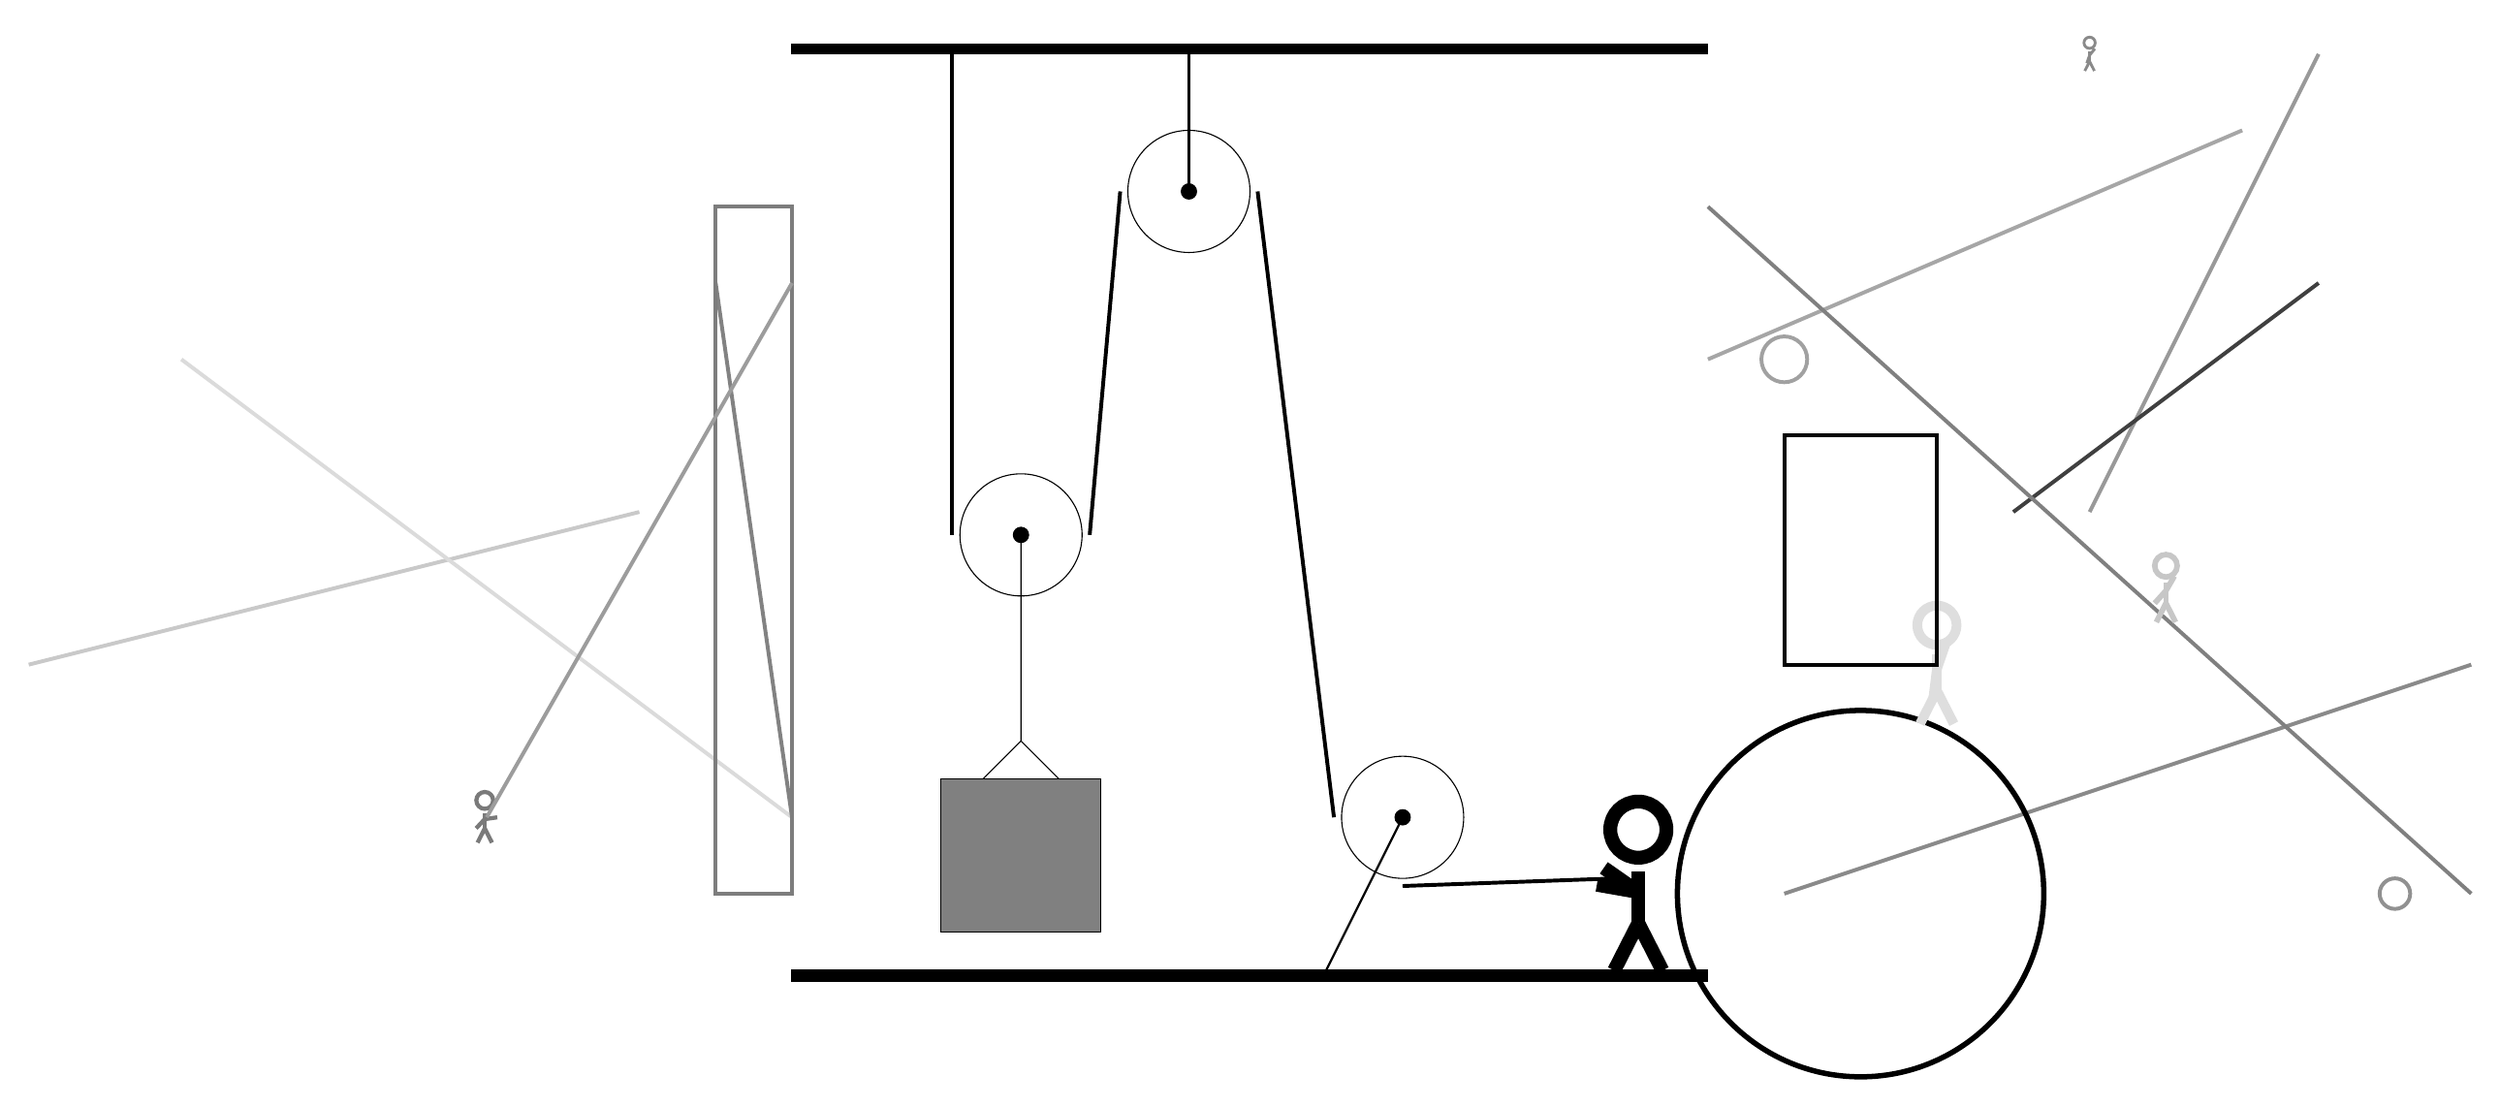
\begin{tikzpicture}
			%%%%% START %%%%%
			
			\draw[fill=black] (-2, 9) rectangle (10, 9.125);
			
			\draw[line width=0.5mm, color=black!12](11, 2) -- (11, 1);
			
			\draw[line width=0.5mm, color=black!21](-4, 3) -- (-12, 1);
			\draw[line width=0.5mm, color=black!46](11, -2) -- (20, 1);
			\draw [line width=0.7mm, color=black!100](12, -2) circle (2.4);
			\draw[line width=0.5mm, color=black!14](-2, -1) -- (-10, 5);
			\node[line width=0.2mm, color=black!46] at (15, 9) {\Strichmaxerl[2][71][51]};
			\draw [line width=0.5mm, color=black!37](11, 5) circle (0.3);
			
			\draw[line width=0.5mm, color=black!49](-2, -1) -- (-3, 6);
			\draw [line width=0.2mm, color=black!19](-2, -1) circle (0.0);
			\node[line width=0.6mm, color=black!13] at (13, 1) {\Strichmaxerl[7][83][71]};
			\draw[line width=0.5mm, color=black!40](15, 3) -- (18, 9);
			\draw[line width=0.5mm, color=black!98] (11, 4) rectangle (13, 1);
			\node[line width=0.4mm, color=black!52] at (-6, -1) {\Strichmaxerl[3][47][8]};
			
			\draw[line width=0.5mm, color=black!75](14, 3) -- (18, 6);
			\draw[line width=0.5mm, color=black!35](10, 5) -- (17, 8);
			\draw [line width=0.2mm, color=black!26](18, 3) circle (0.0);
			
			\draw [line width=0.5mm, color=black!43](19, -2) circle (0.2);
			\draw[line width=0.5mm, color=black!51] (-2, 7) rectangle (-3, -2);
			\draw[line width=0.5mm, color=black!50](10, 7) -- (20, -2);
			\draw[line width=0.5mm, color=black!39](-2, 6) -- (-6, -1);
			\node[line width=0.6mm, color=black!22] at (16, 2) {\Strichmaxerl[4][48][60]};
			
			
			\draw (3.2, 7.2) circle (0.8);
			\draw[fill=black] (3.2, 7.2) circle (0.1);
			\draw[thick] (3.2, 7.2) -- (3.2, 9);
			
			\draw (6, -1) circle (0.8);
			\draw[fill=black] (6, -1) circle (0.1);
			\draw[thick] (6, -1) -- (5, -3);
			
			\draw (1, 2.7) circle (0.8);
			\draw[fill=black] (1, 2.7) circle (0.1);
			
			\draw (1, 2.7) -- (1, 0) -- (0.5, -0.5);
			\draw (1, 0) -- (1.5, -0.5);
			\draw[fill=black!50] (-0.05, -0.5) rectangle (2.05, -2.5);
			
			\draw[line width=0.5mm] (0.1, 9) -- (0.1, 2.7);
			\centerarc[line width=0.5mm](1, 2.7)(180:360:0.9);
			\draw[line width=0.5mm](1.9, 2.7) -- (2.3, 7.2);
			\centerarc[line width=0.5mm](3.2, 7.2)(0:180:0.9);
			\draw[line width=0.5mm](4.1, 7.2) -- (5.1, -1);
			\centerarc[line width=0.5mm](6, -1)(180:270:0.9);
			\draw[line width=0.5mm](6, -1.9) -- (8.8, -1.8);
			
			\node at (9, -1.9) {\Strichmaxerl[10][-35][170]};
			
			\draw[fill=black] (-2, -3) rectangle (10, -3.15);
			
			%%%%% END %%%%%
		\end{tikzpicture}
	\end{figure}	
\end{document}